\documentclass[
11pt, % The default document font size, options: 10pt, 11pt, 12pt
%codirector, % Uncomment to add a codirector to the title page
]{charter} 


% El títulos de la memoria, se usa en la carátula y se puede usar el cualquier lugar del documento con el comando \ttitle
\titulo{Predicción del NDVI de cebada con series temporales de Sentinel-2 e Inteligencia Artificial} 

% Nombre del posgrado, se usa en la carátula y se puede usar el cualquier lugar del documento con el comando \degreename
%\posgrado{Carrera de Especialización en Sistemas Embebidos} 
%\posgrado{Carrera de Especialización en Internet de las Cosas} 
\posgrado{Carrera de Especialización en Inteligencia Artificial}
%\posgrado{Maestría en Sistemas Embebidos} 
%\posgrado{Maestría en Internet de las cosas}

% Tu nombre, se puede usar el cualquier lugar del documento con el comando \authorname
% IMPORTANTE: no omitir titulaciones ni tildación en los nombres, también se recomienda escribir los nombres completos (tal cual los tienen en su documento)
\autor{Dr. Ing. Agr. Adrián Lapaz Olveira}

% El nombre del director y co-director, se puede usar el cualquier lugar del documento con el comando \supname y \cosupname y \pertesupname y \pertecosupname
\director{Esp. Ing. Maria Carina Roldán}
\pertenenciaDirector{FIUBA} 
\codirector{Ing. Ariadna Garmendia} % para que aparezca en la portada se debe descomentar la opción codirector en los parámetros de documentclass
\pertenenciaCoDirector{FIUBA}

% Nombre del cliente, quien va a aprobar los resultados del proyecto, se puede usar con el comando \clientename y \empclientename
\cliente{Ph.D. Ing. Agr. Andrés Berger}
\empresaCliente{INIA}
 
\fechaINICIO{11 de marzo de 2025}		%Fecha de inicio de la cursada de GdP \fechaInicioName
\fechaFINALPlan{22 de abril de 2025} 	%Fecha de final de cursada de GdP
\fechaFINALTrabajo{31 de agosto de 2025}	%Fecha de defensa pública del trabajo final


\begin{document}

\maketitle
\thispagestyle{empty}
\pagebreak


\thispagestyle{empty}
{\setlength{\parskip}{0pt}
\tableofcontents{}
}
\pagebreak


\section*{Registros de cambios}
\label{sec:registro}


\begin{table}[ht]
\label{tab:registro}
\centering
\begin{tabularx}{\linewidth}{@{}|c|X|c|@{}}
\hline
\rowcolor[HTML]{C0C0C0} 
Revisión & \multicolumn{1}{c|}{\cellcolor[HTML]{C0C0C0}Detalles de los cambios realizados} & Fecha      \\ \hline
0      & Creación del documento                                 &\fechaInicioName \\ \hline
%1      & Se completa hasta el punto 5 inclusive                & {día} de {mes} de 202X \\ \hline
%2      & Se completa hasta el punto 9 inclusive
%		  Se puede agregar algo más \newline
%		  En distintas líneas \newline
%		  Así                                                    & {día} de {mes} de 202X \\ \hline
%3      & Se completa hasta el punto 12 inclusive                & {día} de {mes} de 202X \\ \hline
%4      & Se completa el plan	                                 & {día} de {mes} de 202X \\ \hline

% Si hay más correcciones pasada la versión 4 también se deben especificar acá

\end{tabularx}
\end{table}

\pagebreak



\section*{Acta de constitución del proyecto}
\label{sec:acta}

\begin{flushright}
Buenos Aires, \fechaInicioName
\end{flushright}

\vspace{2cm}

Por medio de la presente se acuerda con el \authorname\hspace{1px} que su Trabajo Final de la \degreename\hspace{1px} se titulará ``\ttitle'' y consistirá en la predicción temprana del NDVI máximo de los cultivos de cebada, utilizando series temporales de datos Sentinel-2 y modelos de Inteligencia Artificial para las campañas 2023-2025. El trabajo tendrá un presupuesto preliminar estimado de 600 horas y está financiado por un proyecto de Articulación Academia - Sector Productivo de ANNI (INIA - Ambev, UY), con fecha de inicio el \fechaInicioName\hspace{1px} y fecha de presentación pública el \fechaFinalName.

Se adjunta a esta acta la planificación inicial.

\vfill

% Esta parte se construye sola con la información que hayan cargado en el preámbulo del documento y no debe modificarla
\begin{table}[ht]
\centering
\begin{tabular}{ccc}
\begin{tabular}[c]{@{}c@{}}Dr. Ing. Ariel Lutenberg \\ Director posgrado FIUBA\end{tabular} & \hspace{2cm} & \begin{tabular}[c]{@{}c@{}}\clientename \\ \empclientename \end{tabular} \vspace{2.5cm} \\ 
\multicolumn{3}{c}{\begin{tabular}[c]{@{}c@{}} \supname \\ Director del Trabajo Final\end{tabular}} \vspace{2.5cm} \\
\end{tabular}
\end{table}

\pagebreak



\section{1. Descripción técnica-conceptual del proyecto a realizar}
\label{sec:descripcion}

Este proyecto será realizado por el Dr. Ing. Agr. Adrián Lapaz Olveira como un requisito curricular de la Especialización en Inteligencia Artificial (FIUBA) y será desarrollado en el marco de su investigación en la inicitiva Articulación Academia - Sector Productivo de ANNI denominada \emph{“Desarrollo e implementación de recomendaciones de manejo dinámicas durante el crecimiento del cultivo, basadas en análisis de la base de datos de campo de AB-InBev”}. El desarrollo del proyecto será bajo la dirección de la \supname y la codirección de la \cosupname; ambas docentes de dicha especialización, y la colaboración de investigadores de INIA; PhD. MSc. Ing. Agr. Andrés Berger (cliente), PhD. MSc. Ing. Agr. José Paruelo y Dr. Ing. Agr. Sebastian Mazzilli.

\subsection{Antecedentes}
\label{sec:descripcion}
La producción de cebada (\emph{Hordeum vulgare L.}) con destino industrial tiene como objetivo maximizar el rendimiento con una concentración de proteína en grano del 9 al 12 \%. Para alcanzar este objetivo, se requiere de un diagnóstico nutricional que sea preciso; evitar sub o sobredosis de fertilizantes, y temprano; crecimiento sin restricciones. No obstante, la principal dificultad para alcanzar este objetivo es la falta de precisión en el diagnóstico actual, ya que, al estar basado en determinaciones a la siembra, emergencia y/o estadíos iniciales del cultivo, éste no contempla cómo los factores climáticos afectan el crecimiento de plantas, generando cambios en el rendimiento potencial y en la demanda nutricional futura. Por lo tanto, el diagnóstico nutricional actual de cebada demanda herramientas complementarias que permitan proyectar el crecimiento potencial del cultivo. 

Una de las herramientas calibradas para proyectar el crecimiento de los cultivos es la función $\beta$. Al modelar la acumulación de biomasa según los días desde la siembra (DDS), sus parámetros son biológicamente interpretables facilitando su adpoción en modelos de similación de cultivos. Sin embargo, su parametrización demanda determinaciones de biomasa durante el desarrollo fenólogico siendo esto una desventaja para su adopción por parte de los productores y asesores. La determinación de la biomasa consiste en colectar plantas a campo para luego secarlas en laboratorio, por consiguiente, su imperatividad demanda mucho tiempo, es costosa y tiene limitada representativadad a escala de chacra. Por lo tanto, el uso de indicadores relacionados a la biomasa permitiría proyectar el crecimiento del cultivo a través del ajuste de una función $\beta$ y en consecuencia, predecir la demanda nutricional futura.

La disponibilidad de tecnologías emergentes de teledetección satelital permite estimar \emph{in situ} diversos parámetros biofísicos y químicos de los cultivos de forma rápida, sin costos y a escala de chacra. En esta línea, el uso de datos abiertos de la misión satelital de Sentinel-2 observa la energía electromagnética terrestre a una alta resolución temporal ($\mathbb{<}7$ días), espectral (+3 bandas) y espacial ($10$ o $20$ m de píxel cuadrado), permitiría proyectar de forma precisa el crecimiento del cultivo. Específicamente, estas observaciones se utilizan para caluclar el Índice de Vegetación de Diferencia Normalizada (NDVI) que es un indicador directo del vigor de las plantas, y en efecto un estimador de los parámetros biofísicos de los cultivos. Por lo tanto, si el NDVI presenta una dinámica similar a la acumulación de la biomasa, su proyección con la función $\beta$ aumentaría la precisión del diagnóstico nutricional al estimar el crecimiento potencial del cultivo.

Para llevar a cabo este ajuste de la función $\beta$ y estimar sus parámetros a partir de observaciones iniciales de NDVI, resulta particularmente sólido utilizar la inferencia bayesiana. Bajo este enfoque, se parte de un conocimiento inicial acerca de los parámetros (representado por un \emph{prior}) y se actualiza dicha información conforme se obtienen más mediciones de NDVI a lo largo del ciclo de cultivo. De esta manera, la distribución posterior de los parámetros de la función $\beta$ va reduciendo su dispersión aumentando la precisión en la proyección del NDVI. Este proceso no solo aprovecha los datos iniciales para predecir el crecimiento potencial, sino que también permite incorporar ajustes a medida que surgen nuevas observaciones de NDVI. Por lo tanto, la precisión del enfoque bayesiano para predecir el NDVI potencial del cultivo aumenta con el ciclo fenológico, y en efecto, también la precisión del diagnóstico nutricional.

En la actualidad, la inteligencia artificial está siendo utilizada exitosamente para monitorear diversos parámetros biofísicos y químicos en cultivos y pasturas. Estudios previos han utilizado eficazmente datos históricos de NDVI, temperaturas y precipitación para predecir valores futuros del índice. En esta línea de investigación, un estudio reportó que las Redes Neuronales Artificiales (ANN) predicen con precisión el NDVI futuro de maíz (\emph{Zea mays L.}) en el corto plazo (5-15 días). En este estudio, las ANN fueron entrenadas con el NDVI, índice de diferencia de agua normalizado (NDWI), precipitaciones acumuladas (GPM) y grados días acumulados (AGDD).  Cabe mencionar, que además de estas variables agroclimáticas existen otras que determinan el crecimiento de la cebada, como lo son el coeficiente fototermal (Q) y fotoperíodo (P). También son determinantes las variables de manejo como el cultivar, fecha de siembra y dosis de nitrógeno (N). Por otro lado, en pasturas de campo natural se ha demostrado que el NDVI puede ser predicho en el largo plazo (1-3 meses). Esto se ha logrado a través de desarrollo de modelo híbridos, que combinan modelos paramétricos sigmoideos, similares a la función $\beta$, y algoritmos de ANN. Por lo tanto, las ANN permitirían proyectar el NDVI potencial de la cebada con la integración de los parámetros ajustados de la función $\beta$, variables agroclimáticas y de manejo, aumentando la precisión en el diagnóstico nutricional del cultivo.

En resumen, el NDVI es un fiel indicador del crecimiento de las plantas y su predicción temprana incrementaría la precisión del diagnóstico nutricional. Sin embargo, su proyección durante el ciclo del cultivo no ha investigada en profundidad. Por lo tanto, este trabajo tiene como objetivo i) la predecir el NDVI máximo del cultivo a partir de observaciones que van desde la siembra hasta los 45, 60 y 75 DDS, y ii) evaluar si las variables agroclimáticas y de manejo contribuyen a mejorar la precisión en la estimación del índice (Bayes vs ANN).

\subsection{Metodología}
\label{sec:descripcion}
La Figura 1 muestra el diagrama de flujo de trabajo para predecir el NDVI potencial de lotes comerciales de producción de cebada con destino industrial durante las campañas 2023 y 2024. La información inicial son polígonos georreferencias (JSON) con información de fecha de siembra, cultivar y dosis de N (kg ha\textsuperscript{-1}). A partir de éstos, se recolectarán paralelamente de datos meteorológicos y satelitales.  Luego de recolectadas las observaciones, los datos se particionarán según su destino de análisis; calibración (cebada 2023) y testeo (cebada 2024).  Durante la modelación y el testeo, se utilizarán conjuntos de datos truncados temporalmente a los 45, 60 y 75 DDS. Las predicciones de los modelos se realizarán empleando la información disponible hasta cada uno de estos límites temporales. El modelado bayesiano consistirá en predecir el NDVI potencial a partir de un prior de los parámetros de la curva $\beta$ y las observaciones de NDVI obtenidas en los tres conjuntos de datos truncados (NDVI$_{45/60/75}$). Por otro lado, para cada uno de los tres períodos mencionados, el entrenamiento de la ANN se dividirán datos de entrenamiento (75 \%) y de validación (25 \%) aleatoriamente para una validación cruzada de 4 subconjuntos rotativos. La información para entrenar estas redes será la agroclimática, de manejo y del NDVI diario estimado con la función $\beta$ como $X_i$ y como $y$ el parámetro de N wmax obtenido en la parametrización. Una vez terminada la etapa de calibración de los modelos, se realizará un testeo para cada uno de los períodos de predicción utilizando los datos de la cebada 2024, donde se calcularán las métricas de error predictivo según el NDVI potencial predicho y el observado.   


\begin{figure}[htpb]
\centering 
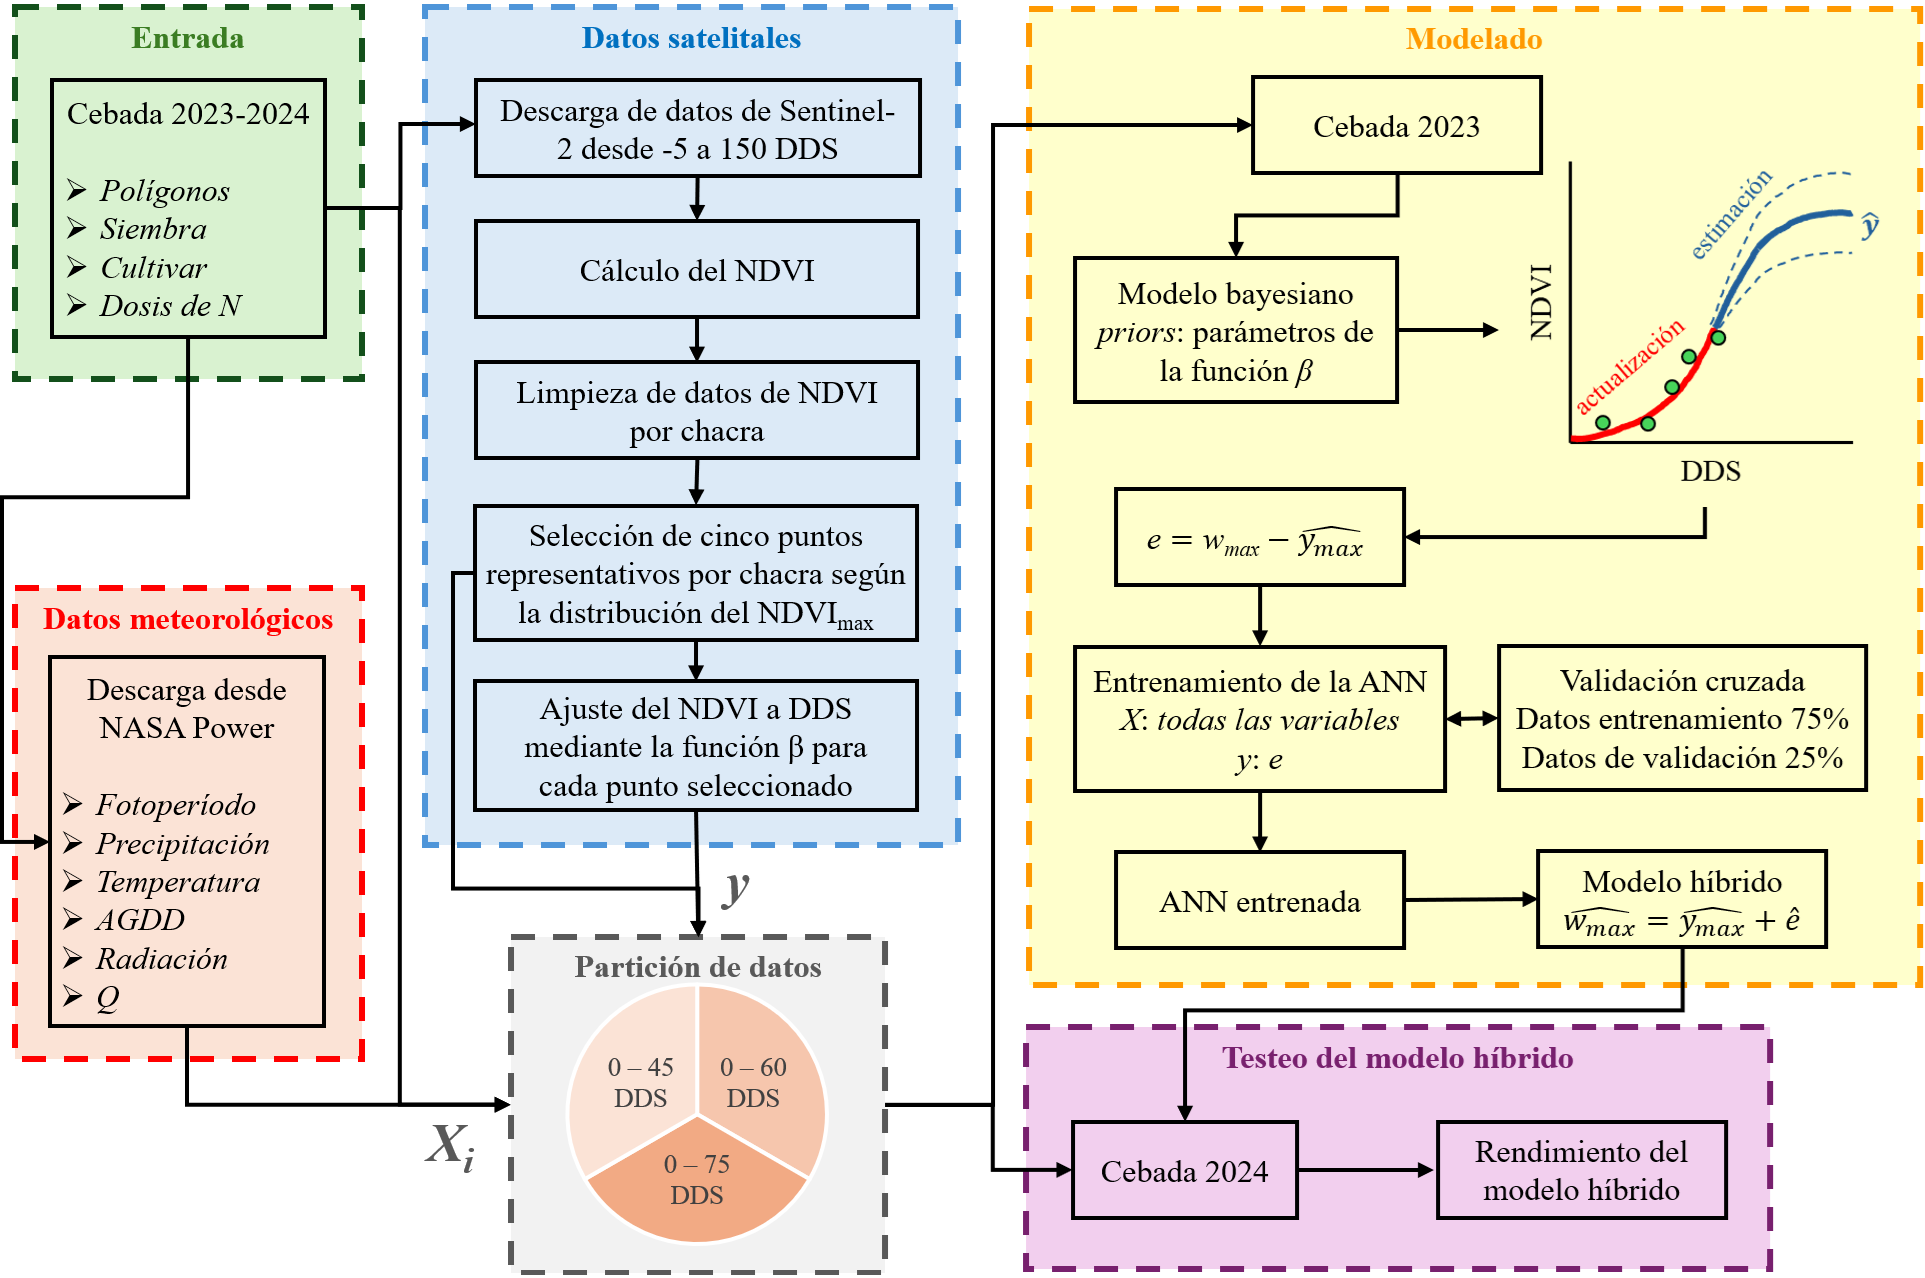
\includegraphics[width=.95\textwidth]{./Figuras/Flujo_de_Trabajo.png}
\caption{Diagrama del flujo de trabajo}
\label{fig:Flujo_de_Trabajo}
\end{figure}


\subsubsection{Datos agrometeorológicos}
\label{sec:descripcion}
Los datos agrometeorológicos serán descargados desde NASA power utilizando el centroide de cada chacra. Las varaibles que se obtendrán diariamente registros de precipitación (PP), temperatura (T), fotoperíodo (P) y radición (R). A partir de estos se calcuilarán la GPM, los AGDD y el Q para cada día ($i$-ésimo) hasta el último día disponible ($n$):

\begin{equation}
\label{eq:GPM}
\text{GPM} = \sum_{i=1}^{n} PP_{i}
\end{equation}

\begin{equation}
\label{eq:AGDD}
\text{AGDD} = \sum_{i=1}^{n} GDD_{i}
\end{equation}

\begin{equation}
\label{eq:Q}
Q_i = \frac{R_i}{T_i - T_{\text{base}}}
\end{equation}


\subsubsection{Datos satelitales}
\label{sec:descripcion}

Para este estudio bianual y de extensa cobertura, se utilizará la plataforma Google Earth Engine para el procesamiento eficiente de los datos de reflectancia de nivel 2-A armonizados del satélite Sentinel-2. Este nivel de producto se caracteriza por correcciones geométricas y radiométricas pre-aplicadas, presentando una precisión posicional nominal de 3 metros y una resolución radiométrica de 12 bits. Para obtener estos datos, en cada chacra se creará un grilla de puntos distanciados cada 10 m. A partir de estas observaciones, se calculará el NDVI como la diferencia normalizada entre la reflectancia ($\alpha$) en el infrarrojo cercano (833 nm, $\pm$ 106 nm, pixel 10 m) y en el rojo (665 nm, $\pm$ 31 nm, pixel 10 m). 

\begin{equation}
\text{NDVI} = \frac{\alpha_{\text{infrarrojo}} - \alpha_{\text{rojo}}}{\alpha_{\text{infrarrojo}} + \alpha_{\text{rojo}}} \label{eq:ndvi_def}
\end{equation}

Una vez calculado el NDVI en cada punto de la grilla, se seleccionaran los cinco más representativos clasificando sus máximos valores registrado en quantiles. Entonces, en cada chacra estos puntos representarán el mínimo, cuantil dos, tres y cuatro, y el máximo, del conjunto de datos con los máximos valores NDVI alcanzados. Esto se para obtener una representatividad de la variación del NDVI potencial a escala de lote.  


\subsubsection{Función $\beta$}
\label{sec:descripcion}

Dado que el comportamiento del NDVI a lo largo del ciclo de crecimiento del cultivo presenta una dinámica similar a la de las plantas, se ajustará la función $\beta$ porque modela con precisión la acumulación de biomasa en función de los DDS. A diferencia de otros modelos sigmoides, esta función incorpora parámetros biológicamente interpretables, como se muestra en la Figura \ref{fig:Curva_Beta }. Además, su estructura matemática permite modelar de manera continua la evolución de la biomasa sin generar discontinuidades en la transición entre fases de crecimiento, proporcionando estimaciones más realistas y ajustadas a la naturaleza determinante del crecimiento de estos cultivos. Por lo tanto, la parametrización de la dinámica del NDVI mediante la función $\beta$ ofrece una estrategia promisoria para la proyección temprana de la biomasa acumulada en cebada.

\begin{figure}[htpb]
    \centering
    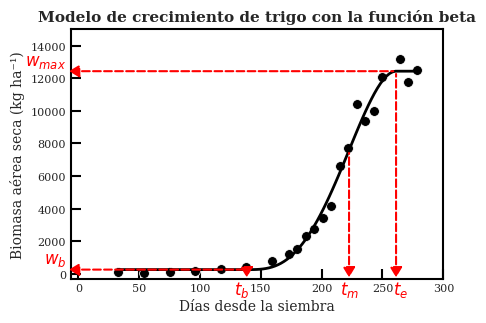
\includegraphics[width=.5\textwidth]{./Figuras/Curva_Beta.png}
    \caption{Dinámica temporal observada (puntos) y ajustada mediante la función de crecimiento beta (curva) de la biomasa aérea seca en trigo de invierno (datos de Gregory et al., 1978). Los parámetros de la función beta son los siguientes, $w_b$: biomasa inicial; $w_{\max}$: biomasa máxima alcanzada; $t_b$: tiempo de inicio del crecimiento significativo; $t_m$: punto de inflexión (tasa de crecimiento máxima); $t_e$: tiempo en el que finaliza el crecimiento.}
    \label{fig:Curva_Beta }
\end{figure}



Estos parámetros permiten describir con precisión el patrón sigmoide del crecimiento, caracterizando tanto la fase inicial lenta, como el período de rápido crecimiento y la fase final de estabilización. 

La ecuación para calcular estos parámetros mediante mínimos cuadrados no lineales (nls) es la siguiente

\begin{equation}
\label{eq:betaGrowth}
w = w_b \;+\; \bigl(w_{\max} - w_b\bigr) 
        \left(1 + \frac{t_e - t}{t_e - t_m}\right)
        \left(\frac{t - t_b}{t_e - t_b}\right)^{\!\frac{t_m - t_b}{t_e - t_m}}
\end{equation}

sujeto a la condición \(t_b \;\leq\; t_m \;<\; t_e\).


\section{2. Identificación y análisis de los interesados}
\label{sec:interesados}

\begin{table}[ht]
\caption{Identificación de los interesados}
\label{tab:interesados}
\begin{tabularx}{\linewidth}{@{}|l|X|X|X|@{}} 
\hline
\rowcolor[HTML]{C0C0C0} 
Rol           & Nombre y Apellido & Organización  & Puesto         \\ \hline
Auspiciante   &   	    -		  & 	   -  	  &     -  	       \\ \hline
Cliente       & \clientename      & \empclientename & Investigador \\ \hline
Impulsor      & \clientename      & \empclientename & Investigador \\ \hline
Responsable   & \authorname       & FIUBA         & Alumno         \\ \hline
Colaboradores & PhD. MSc. Ing. Agr. José Paruelo \newline
				Dr. Ing. Agr. Sebastian Mazzilli  & INIA  \newline
													INIA  & Investigador  \newline
													        Investigador \\ \hline
Orientadores  & \supname \newline 
                \cosupname       & \pertesupname \newline
                				   \pertecosupname  & Director del Trabajo Final \newline 
                                                      Co-Director del Trabajo Final \\ \hline

% NO PUDE ASIGNAR MIEMBROS Y LUEGOS LLAMARLOS EN LA TABLA
%Equipo        & \miembro1 \newline 
%				\miembro2          &              	&        	\\ \hline

Equipo        & 	   -		 & 	     -		 & 	     -		  \\ \hline
Opositores    & 	   -		 & 	     -		 & 	     -		  \\ \hline
Usuario final & 	   -		 & 	     -		 & 	     -		  \\ \hline
\end{tabularx}
\end{table}


\section{3. Propósito del proyecto}
\label{sec:proposito}

Este proyecto busca desarrollar una herramienta complementaría al diagnóstico nutricional actual de cebada que permita estimar indicadores, como el NDVI, del crecimiento potencial de los cultivos. Esto permitiría a los productores desarrollar estrategias de manejos anticipadas, evitando pérdidas en el rendimiento potencial del cultivo y alcanzado una concentración de proteína en grano óptima para la calidad maltera. 


\section{4. Alcance del proyecto}
\label{sec:alcance}

En este proyecto se incluye información sobre los sistemas productivos de cebada con destino industrial para la empresa AmBev. Dada las limitaciones en tiempo para realizar el proyecto dentro del contexto académico de la especialización, no se incluyen información de la producción de cebada 2025 y mediciones de biomasa realizadas en 2024 y 2025.

El proyecto incluye:
\begin{itemize}
	\item Información georeferencia de la producción de cebada 2023 y 2024 para miles de chacras.
		\begin{itemize}
		\item Polígono de la chacra.
		\item Fecha de siembra
		\item Cultivar.
		\item Aplicación de fertilizantes		
		\end{itemize}
	\item Datos agroclimáticos por chacra
		\begin{itemize}
		\item Precipitación.
		\item Temperatura diaria.
		\item Fotoperíodo.
		\item Grados días.
		\item Radiación.
		\item Coeficiente fototermal		
		\end{itemize}
	\item Datos satelitales para cinco puntos representativos por chacra
		\begin{itemize}
		\item NDVI.
		\item Parámetros de la cruva $\beta$.
		\end{itemize}
	
\end{itemize}

El presente proyecto no incluye información sobre el corriente año (2025) y 60 observaciones realizadas en chacras que produjeron cebada en el 2024, y otras mediciones que se realizarán en el 2025, porque la dimensión del proyecto está acotada a la aplicación de la inteligencia artificial en datos de teledetección. No obstante, se podrían incluir los datos 2024 para ver si el NDVI estimado se correlaciona con las variables observadas que son:
\begin{itemize}
	\item Observaciones en espigazón.
		\begin{itemize}
		\item Biomasa aérea seca y fresca.
		\item Concentración y acumulación de nitrógeno en la biomasa.
		\item Índice de nutrición nitrogenada (INN).
		\item Índice de diagnóstico hídrico (WDI).		
		\end{itemize}
	\item Observados en cosecha.
		\begin{itemize}
		\item Rendimiento en grano.
		\item Concentración y acumulación de nitrógeno en grano.
		\item Proteína en grano.
		\item Índice de cosecha.
		\item Calidad de grano.
		\end{itemize}
	
\end{itemize}



\section{5. Supuestos del proyecto}
\label{sec:supuestos}

Para el desarrollo del presente proyecto se supone que:

\begin{itemize}
	\item Se dispondrá de la asesoría de expertos en la tematica de agronomía, computación y percepción remota.
	\item El tiempo requerido para el entrenamiento de modelos será adecuado para cumplir con los requisitos curriculares de la especialización.
	\item La financiación del proyecto ya está cubierta por las instituciones del estudiante.
\end{itemize}



\section{6. Requerimientos}
\label{sec:requerimientos}

\begin{consigna}{red} % ELIMINAR \begin{consigna}{red} y \end{consigna}{red} en las secciones que vayan completando para cada entrega parcial.
Los requerimientos deben enumerarse y de ser posible estar agrupados por afinidad, por ejemplo:

\begin{enumerate}
	\item Requerimientos funcionales:
		\begin{enumerate}
			\item El sistema debe...
			\item Tal componente debe...
			\item El usuario debe poder...
		\end{enumerate}
	\item Requerimientos de documentación:
		\begin{enumerate}
			\item Requerimiento 1.
			\item Requerimiento 2 (prioridad menor)
		\end{enumerate}
	\item Requerimiento de testing...
	\item Requerimientos de la interfaz...
	\item Requerimientos interoperabilidad...
	\item etc...
\end{enumerate}

Leyendo los requerimientos se debe poder interpretar cómo será el proyecto y su funcionalidad.

Indicar claramente cuál es la prioridad entre los distintos requerimientos y si hay requerimientos opcionales. 

\textbf{¡¡¡No olvidarse de que los requerimientos incluyen a las regulaciones y normas vigentes!!!}

Y al escribirlos seguir las siguientes reglas:
\begin{itemize}
	\item Ser breve y conciso (nadie lee cosas largas). 
	\item Ser específico: no dejar lugar a confusiones.
	\item Expresar los requerimientos en términos que sean cuantificables y medibles.
\end{itemize}

\end{consigna} % ELIMINAR \begin{consigna}{red} y \end{consigna}{red} en las secciones que vayan completando para cada entrega parcial.

\section{7. Historias de usuarios (\textit{Product backlog})}
\label{sec:backlog}

\begin{consigna}{red}
Descripción: en esta sección se deben incluir las historias de usuarios y su ponderación (\textit{history points}). Recordar que las historias de usuarios son descripciones cortas y simples de una característica contada desde la perspectiva de la persona que desea la nueva capacidad, generalmente un usuario o cliente del sistema. La ponderación es un número entero que representa el tamaño de la historia comparada con otras historias de similar tipo.

Se debe indicar explícitamente el criterio para calcular los \textit{story points} de cada historia.

El formato propuesto es: 
\begin{enumerate}
\item ``Como [rol] quiero [tal cosa] para [tal otra cosa]."

\textit{Story points}: 8 (complejidad: 3, dificultad: 2, incertidumbre: 3)
\end{enumerate}
\end{consigna}

\section{8. Entregables principales del proyecto}
\label{sec:entregables}

\begin{consigna}{red}
Los entregables del proyecto son (ejemplo):

\begin{itemize}
	\item Manual de usuario.
	\item Diagrama de circuitos esquemáticos.
	\item Código fuente del firmware.
	\item Diagrama de instalación.
	\item Memoria del trabajo final.
	\item etc...
\end{itemize}
\end{consigna}

\section{9. Desglose del trabajo en tareas}
\label{sec:wbs}

\begin{consigna}{red}
El WBS debe tener relación directa o indirecta con los requerimientos.  Son todas las actividades que se harán en el proyecto para dar cumplimiento a los requerimientos. Se recomienda mostrar el WBS mediante una lista indexada:

\begin{enumerate}
\item Grupo de tareas 1 (suma h)
	\begin{enumerate}
	\item Tarea 1 (tantas h)
	\item Tarea 2 (tantas h)
	\item Tarea 3 (tantas h)
	\end{enumerate}
\item Grupo de tareas 2 (suma h)
	\begin{enumerate}
	\item Tarea 1 (tantas h)
	\item Tarea 2 (tantas h)
	\item Tarea 3 (tantas h)
	\end{enumerate}
\item Grupo de tareas 3 (suma h)
	\begin{enumerate}
	\item Tarea 1 (tantas h)
	\item Tarea 2 (tantas h)
	\item Tarea 3 (tantas h)
	\item Tarea 4 (tantas h)
	\item Tarea 5 (tantas h)
	\end{enumerate}
\end{enumerate}

Cantidad total de horas: tantas.

\textbf{¡Importante!:} la unidad de horas es h y va separada por espacio del número. Es incorrecto escribir ``23hs".

\textbf{Se recomienda que no haya ninguna tarea que lleve más de 40 h.} De ser así se recomienda dividirla en tareas de menor duración.

\end{consigna}

\section{10. Diagrama de Activity On Node}
\label{sec:AoN}

\begin{consigna}{red}
Armar el AoN a partir del WBS definido en la etapa anterior.

Una herramienta simple para desarrollar los diagramas es el Draw.io (\url{https://app.diagrams.net/}).
\href{https://app.diagrams.net}{Draw.io}


\begin{figure}[htpb]
\centering 
\includegraphics[width=.8\textwidth]{./Figuras/AoN.png}
\caption{Diagrama de \textit{Activity on Node}.}
\label{fig:AoN}
\end{figure}

Indicar claramente en qué unidades están expresados los tiempos.
De ser necesario indicar los caminos semi críticos y analizar sus tiempos mediante un cuadro.
Es recomendable usar colores y un cuadro indicativo describiendo qué representa cada color.

\end{consigna}

\section{11. Diagrama de Gantt}
\label{sec:gantt}

\begin{consigna}{red}
Existen muchos programas y recursos \textit{online} para hacer diagramas de Gantt, entre los cuales destacamos:

\begin{itemize}
\item Planner
\item GanttProject
\item Trello + \textit{plugins}. En el siguiente link hay un tutorial oficial: \\ \url{https://blog.trello.com/es/diagrama-de-gantt-de-un-proyecto}
\item Creately, herramienta online colaborativa. \\\url{https://creately.com/diagram/example/ieb3p3ml/LaTeX}
\item Se puede hacer en latex con el paquete \textit{pgfgantt}\\ \url{http://ctan.dcc.uchile.cl/graphics/pgf/contrib/pgfgantt/pgfgantt.pdf}
\end{itemize}

Pegar acá una captura de pantalla del diagrama de Gantt, cuidando que la letra sea suficientemente grande como para ser legible. 
Si el diagrama queda demasiado ancho, se puede pegar primero la ``tabla'' del Gantt y luego pegar la parte del diagrama de barras del diagrama de Gantt.

Configurar el software para que en la parte de la tabla muestre los códigos del EDT (WBS).\\
Configurar el software para que al lado de cada barra muestre el nombre de cada tarea.\\
Revisar que la fecha de finalización coincida con lo indicado en el Acta Constitutiva.

En la figura \ref{fig:gantt}, se muestra un ejemplo de diagrama de gantt realizado con el paquete de \textit{pgfgantt}. 
En la plantilla pueden ver el código que lo genera y usarlo de base para construir el propio.

Las fechas pueden ser calculadas utilizando alguna de las herramientas antes citadas. Sin embargo, el siguiente ejemplo
fue elaborado utilizando 
\href{https://docs.google.com/spreadsheets/d/1fBz8NhSpc4tkkhz3KjJCbh1nR_ltDkfEcZi4tZXduqs}{esta hoja de cálculo}.

Es importante destacar que el ancho del diagrama estará dado por la longitud del texto utilizado para las tareas 
(Ejemplo: tarea 1, tarea 2, etcétera) y el valor \textit{x unit}. Para mejorar la apariencia del diagrama, es necesario
ajustar este valor y, quizás, acortar los nombres de las tareas.

\begin{figure}[htpb]
  \begin{center}
    \begin{ganttchart}[
      time slot unit=day,
      time slot format=isodate,
      x unit=0.038cm,
      y unit title=0.7cm,
      y unit chart=0.6cm,
      milestone/.append style={xscale=4}
      ]{2021-03-05}{2021-12-16}
      \gantttitlecalendar*{2021-03-05}{2021-12-16}{year} \\
      \gantttitlecalendar*{2021-03-05}{2021-12-16}{month} \\
      \ganttgroup{Duración Total}{2021-03-05}{2021-12-16} \\
      %%%%%%%%%%%%%%%%%Organización
      \ganttgroup{Organización}{2021-03-05}{2021-04-16} \\
      \ganttbar{Planificación del proyecto}{2021-03-05}{2021-04-15} \\
      %%%%%%%%%%%%%%%%%Ejecución
      \ganttgroup{Ejecución}{2021-04-16}{2021-10-21} \\
      \ganttbar{Tarea 1}{2021-04-16}{2021-04-29} \\
      \ganttbar{Tarea 2}{2021-04-30}{2021-05-13} \\
      \ganttbar{Tarea 3}{2021-05-14}{2021-05-27} \\
      \ganttbar{Tarea 4}{2021-05-28}{2021-07-12} \\
      \ganttbar{Tarea 5}{2021-07-13}{2021-08-09} \\
      \ganttbar{Tarea 6}{2021-08-10}{2021-09-23} \\
      \ganttbar{Tarea 7}{2021-09-24}{2021-09-30} \\
      \ganttbar{Tarea 8}{2021-10-01}{2021-10-14} \\
      \ganttbar{Tarea 9}{2021-10-15}{2021-10-21} \\
      % %%%%%%%%%%%%%%%%%Finalización
      \ganttgroup{Finalización}{2021-10-22}{2021-12-16} \\
      \ganttbar{Memoria v1}{2021-10-22}{2021-11-04} \\
      \ganttbar{Memoria v2}{2021-11-05}{2021-11-18} \\
      \ganttbar{Memoria final}{2021-11-19}{2021-12-02} \\
      % La fecha del siguiente milestone es la fecha en que terminamos la memoria
      \ganttmilestone{Enviar memoria al director}{2021-12-02} \\
      \ganttbar{Elaborar la presentación}{2021-12-03}{2021-12-16} \\
      \ganttmilestone{Ensayo de la presentación}{2021-12-16} \\
      %%%%%%%%%%%%%%%%%%%%%%%%%%%%%%%%%%%%%%%%%%%%%%%%%%%%%%%%%%%%%%%
    \end{ganttchart}
  \end{center}
  \caption{Diagrama de gantt de ejemplo}
  \label{fig:gantt}
\end{figure}


\begin{landscape}
\begin{figure}[htpb]
\centering 
\includegraphics[height=.85\textheight]{./Figuras/Gantt-2.png}
\caption{Ejemplo de diagrama de Gantt (apaisado).} %Modificar este título acorde.
\label{fig:diagGantt}
\end{figure}

\end{landscape}

\end{consigna}


\section{12. Presupuesto detallado del proyecto}
\label{sec:presupuesto}

\begin{consigna}{red}
Si el proyecto es complejo entonces separarlo en partes:
\begin{itemize}
	\item Un total global, indicando el subtotal acumulado por cada una de las áreas.
	\item El desglose detallado del subtotal de cada una de las áreas.
\end{itemize}

IMPORTANTE: No olvidarse de considerar los COSTOS INDIRECTOS.

Incluir la aclaración de si se emplea como moneda el peso argentino (ARS) o si se usa moneda extranjera (USD, EUR, etc). Si es en moneda extranjera se debe indicar la tasa de conversión respecto a la moneda local en una fecha dada.

\end{consigna}

\begin{table}[htpb]
\centering
\begin{tabularx}{\linewidth}{@{}|X|c|r|r|@{}}
\hline
\rowcolor[HTML]{C0C0C0} 
\multicolumn{4}{|c|}{\cellcolor[HTML]{C0C0C0}COSTOS DIRECTOS} \\ \hline
\rowcolor[HTML]{C0C0C0} 
Descripción &
  \multicolumn{1}{c|}{\cellcolor[HTML]{C0C0C0}Cantidad} &
  \multicolumn{1}{c|}{\cellcolor[HTML]{C0C0C0}Valor unitario} &
  \multicolumn{1}{c|}{\cellcolor[HTML]{C0C0C0}Valor total} \\ \hline
 &
  \multicolumn{1}{c|}{} &
  \multicolumn{1}{c|}{} &
  \multicolumn{1}{c|}{} \\ \hline
 &
  \multicolumn{1}{c|}{} &
  \multicolumn{1}{c|}{} &
  \multicolumn{1}{c|}{} \\ \hline
\multicolumn{1}{|l|}{} &
   &
   &
   \\ \hline
\multicolumn{1}{|l|}{} &
   &
   &
   \\ \hline
\multicolumn{3}{|c|}{SUBTOTAL} &
  \multicolumn{1}{c|}{} \\ \hline
\rowcolor[HTML]{C0C0C0} 
\multicolumn{4}{|c|}{\cellcolor[HTML]{C0C0C0}COSTOS INDIRECTOS} \\ \hline
\rowcolor[HTML]{C0C0C0} 
Descripción &
  \multicolumn{1}{c|}{\cellcolor[HTML]{C0C0C0}Cantidad} &
  \multicolumn{1}{c|}{\cellcolor[HTML]{C0C0C0}Valor unitario} &
  \multicolumn{1}{c|}{\cellcolor[HTML]{C0C0C0}Valor total} \\ \hline
\multicolumn{1}{|l|}{} &
   &
   &
   \\ \hline
\multicolumn{1}{|l|}{} &
   &
   &
   \\ \hline
\multicolumn{1}{|l|}{} &
   &
   &
   \\ \hline
\multicolumn{3}{|c|}{SUBTOTAL} &
  \multicolumn{1}{c|}{} \\ \hline
\rowcolor[HTML]{C0C0C0}
\multicolumn{3}{|c|}{TOTAL} &
   \\ \hline
\end{tabularx}%
\end{table}


\section{13. Gestión de riesgos}
\label{sec:riesgos}

\begin{consigna}{red}
a) Identificación de los riesgos (al menos cinco) y estimación de sus consecuencias:
 
Riesgo 1: detallar el riesgo (riesgo es algo que si ocurre altera los planes previstos de forma negativa)
\begin{itemize}
	\item Severidad (S): mientras más severo, más alto es el número (usar números del 1 al 10).\\
	Justificar el motivo por el cual se asigna determinado número de severidad (S).
	\item Probabilidad de ocurrencia (O): mientras más probable, más alto es el número (usar del 1 al 10).\\
	Justificar el motivo por el cual se asigna determinado número de (O). 
\end{itemize}   

Riesgo 2:
\begin{itemize}
	\item Severidad (S): X.\\
	Justificación...
	\item Ocurrencia (O): Y.\\
	Justificación...
\end{itemize}

Riesgo 3:
\begin{itemize}
	\item Severidad (S):  X.\\
	Justificación...
	\item Ocurrencia (O): Y.\\
	Justificación...
\end{itemize}


b) Tabla de gestión de riesgos:      (El RPN se calcula como RPN=SxO)

\begin{table}[htpb]
\centering
\begin{tabularx}{\linewidth}{@{}|X|c|c|c|c|c|c|@{}}
\hline
\rowcolor[HTML]{C0C0C0} 
Riesgo & S & O & RPN & S* & O* & RPN* \\ \hline
       &   &   &     &    &    &      \\ \hline
       &   &   &     &    &    &      \\ \hline
       &   &   &     &    &    &      \\ \hline
       &   &   &     &    &    &      \\ \hline
       &   &   &     &    &    &      \\ \hline
\end{tabularx}%
\end{table}

Criterio adoptado: 

Se tomarán medidas de mitigación en los riesgos cuyos números de RPN sean mayores a...

Nota: los valores marcados con (*) en la tabla corresponden luego de haber aplicado la mitigación.

c) Plan de mitigación de los riesgos que originalmente excedían el RPN máximo establecido:
 
Riesgo 1: plan de mitigación (si por el RPN fuera necesario elaborar un plan de mitigación).
  Nueva asignación de S y O, con su respectiva justificación:
  \begin{itemize}
	\item Severidad (S*): mientras más severo, más alto es el número (usar números del 1 al 10).
          Justificar el motivo por el cual se asigna determinado número de severidad (S).
	\item Probabilidad de ocurrencia (O*): mientras más probable, más alto es el número (usar del 1 al 10).
          Justificar el motivo por el cual se asigna determinado número de (O).
	\end{itemize}

Riesgo 2: plan de mitigación (si por el RPN fuera necesario elaborar un plan de mitigación).
 
Riesgo 3: plan de mitigación (si por el RPN fuera necesario elaborar un plan de mitigación).

\end{consigna}


\section{14. Gestión de la calidad}
\label{sec:calidad}

\begin{consigna}{red}
Elija al menos diez requerimientos que a su criterio sean los más importantes/críticos/que aportan más valor y para cada uno de ellos indique las acciones de verificación y validación que permitan asegurar su cumplimiento.

\begin{itemize} 
\item Req \#1: copiar acá el requerimiento con su correspondiente número.

\begin{itemize}
	\item Verificación para confirmar si se cumplió con lo requerido antes de mostrar el sistema al cliente. Detallar.
	\item Validación con el cliente para confirmar que está de acuerdo en que se cumplió con lo requerido. Detallar. 
\end{itemize}

\end{itemize}

Tener en cuenta que en este contexto se pueden mencionar simulaciones, cálculos, revisión de hojas de datos, consulta con expertos, mediciones, etc.  

Las acciones de verificación suelen considerar al entregable como ``caja blanca'', es decir se conoce en profundidad su funcionamiento interno.  

En cambio, las acciones de validación suelen considerar al entregable como ``caja negra'', es decir, que no se conocen los detalles de su funcionamiento interno.

\end{consigna}

\section{15. Procesos de cierre}    
\label{sec:cierre}

\begin{consigna}{red}
Establecer las pautas de trabajo para realizar una reunión final de evaluación del proyecto, tal que contemple las siguientes actividades:

\begin{itemize}
	\item Pautas de trabajo que se seguirán para analizar si se respetó el Plan de Proyecto original:\\
	 - Indicar quién se ocupará de hacer esto y cuál será el procedimiento a aplicar. 
	\item Identificación de las técnicas y procedimientos útiles e inútiles que se emplearon, los problemas que surgieron y cómo se solucionaron:\\
	 - Indicar quién se ocupará de hacer esto y cuál será el procedimiento para dejar registro.
	\item Indicar quién organizará el acto de agradecimiento a todos los interesados, y en especial al equipo de trabajo y colaboradores:\\
	  - Indicar esto y quién financiará los gastos correspondientes.
\end{itemize}

\end{consigna}

\end{document}